% This is now Chapter 5

The proposed system is a modular, end-to-end multimodal machine learning pipeline that processes audio, video, and transcript data streams in parallel, fuses their representations, and predicts teaching effectiveness using a unified classifier. This architecture leverages state-of-the-art models and best practices from the HuggingFace ecosystem and the broader machine learning community.

\begin{figure}[H]
    \centering
    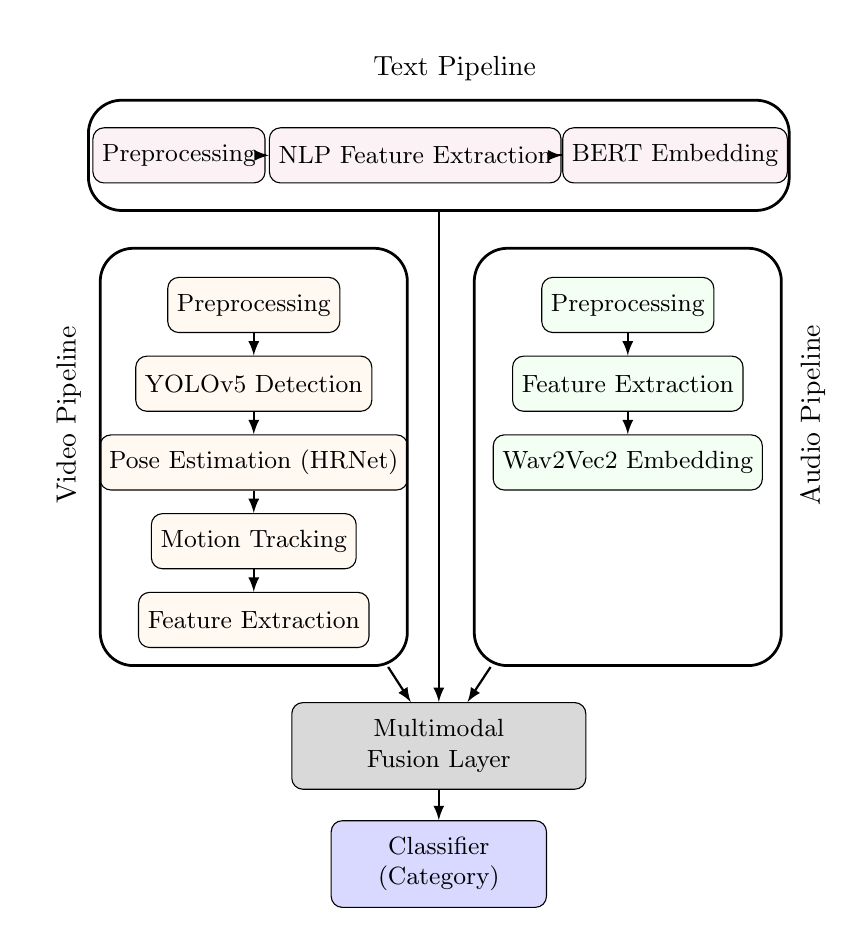
\begin{tikzpicture}[
        module/.style={rectangle, draw, rounded corners, minimum width=2.5cm, minimum height=1.1cm, text width=2.5cm, align=center, font=\small, fill=gray!10},
        arrow/.style={->, thick, >=latex},
        process/.style={rectangle, draw, rounded corners, minimum width=2cm, minimum height=0.7cm, font=\small, fill=white},
        pipelinebox/.style={draw=black, rounded corners=12pt, line width=1pt, minimum width=3.2cm, minimum height=5.3cm}
    ]

        % Text pipeline
        \node[process, fill=purple!5] (t1) at (-6.2,3.3) {Preprocessing};
        \node[process, fill=purple!5] (t2) at (-3.2,3.3) {NLP Feature Extraction};
        \node[process, fill=purple!5] (t3) at (0.1,3.3) {BERT Embedding};
        \node[pipelinebox,rotate=0, minimum width=8.9cm,minimum height=1.4cm, fill=none] (cover3) at (-2.9,3.3) {};
        \node[label, rotate=0, xshift=-2.7cm,yshift=4.4cm] {Text Pipeline};

        % Video pipeline
        \node[process, fill=orange!5] (v1) at (-5.25,1.4) {Preprocessing};
        \node[process, fill=orange!5] (v2) at (-5.25,0.4) {YOLOv5 Detection};
        \node[process, fill=orange!5] (v3) at (-5.25,-0.6) {Pose Estimation (HRNet)};
        \node[process, fill=orange!5] (v4) at (-5.25,-1.6) {Motion Tracking};
        \node[process, fill=orange!5] (v5) at (-5.25,-2.6) {Feature Extraction};
        \node[pipelinebox,minimum width=3.9cm, fill=none] (cover1) at (-5.25,-.53) {};
        \node[label, rotate=90, xshift=0cm,yshift=7.6cm] {Video Pipeline};


        % Audio pipeline
        \node[process, fill=green!5] (a1) at (-0.5,1.4) {Preprocessing};
        \node[process, fill=green!5] (a2) at (-0.5,0.4) {Feature Extraction};
        \node[process, fill=green!5] (a3) at (-0.5,-0.6) {Wav2Vec2 Embedding};
        \node[pipelinebox, minimum width=3.9cm,fill=none] (cover2) at (-0.5,-.53) {};
        \node[label, rotate=90, xshift=0cm,yshift=-1.85cm] {Audio Pipeline};

       

        % Fusion and classifier
        \node[module, fill=gray!30, minimum width=3.5cm, text width=3.5cm] (fusion) at (-2.9,-4.2) {Multimodal Fusion Layer};
        \node[module, fill=blue!15, minimum width=2.5cm, text width=2.5cm] (clf) at (-2.9,-5.7) {Classifier\\(Category)};

        % Arrows for video
        \draw[arrow] (v1) -- (v2);
        \draw[arrow] (v2) -- (v3);
        \draw[arrow] (v3) -- (v4);
        \draw[arrow] (v4) -- (v5);
        \draw[arrow] (cover1) -- (fusion);

        % Arrows for audio
        \draw[arrow] (a1) -- (a2);
        \draw[arrow] (a2) -- (a3);
        \draw[arrow] (cover2) -- (fusion);

        % Arrows for text
        \draw[arrow] (t1) -- (t2);
        \draw[arrow] (t2) -- (t3);
        \draw[arrow] (cover3) -- (fusion);

        % Fusion to classifier
        \draw[arrow] (fusion) -- (clf);

    \end{tikzpicture}
    \centering
    \caption{High-level architecture of the proposed multimodal teacher evaluation system. Each modality is processed by a dedicated pipeline; their features are fused with session metadata and classified.}
    \label{fig:multimodal_architecture}
\end{figure}

\subsection{Video Stream pipeline}  
\begin{itemize}
    \item \textbf{Preprocessing:} Video frames are normalized and denoised.
    \item \textbf{Human Detection:} YOLOv5 (via HuggingFace) detects all people in each frame.
    \item \textbf{Pose Estimation:} HRNet or OpenPose extracts skeletal keypoints for each detected person.
    \item \textbf{Motion Tracking:} Kalman filtering links poses across frames to track teacher movement.
    \item \textbf{Feature Extraction:} Computes gesture frequency, classroom coverage, interaction zones, and movement patterns \cite{mcneill1992hand}.
\end{itemize}

\subsection{Audio Stream pipeline}  
\begin{itemize}
    \item \textbf{Preprocessing:} Audio is denoised and segmented.
    \item \textbf{Feature Extraction:} PRAAT and Python extract prosodic features (pitch, intensity, speech rate) and emotion embeddings.
    \item \textbf{Audio Embedding:} Wav2Vec2 (HuggingFace Transformers) produces deep audio representations.
\end{itemize}

\subsection{Text Stream pipeline}  
\begin{itemize}
    \item \textbf{Preprocessing:} Transcripts are cleaned and tokenized.
    \item \textbf{NLP Feature Extraction:} Sentiment analysis, question type detection, and discourse structure are computed \cite{sinclair1975discourse}.
    \item \textbf{Text Embedding:} BERT or DistilBERT (HuggingFace Transformers) generates semantic embeddings.
\end{itemize}

\subsection{Multimodal Fusion and Classification}  
\begin{itemize}
    \item \textbf{Fusion Layer:} All modality embeddings/features are concatenated and combined with session metadata (e.g., class size, subject).
    \item \textbf{Classifier:} The fused vector is input to a fully connected neural network with a softmax (for categorical) or regression (for continuous) output, predicting teaching effectiveness.
\end{itemize}

\textbf{Modeling and Training:}  
\begin{itemize}
    \item All models are implemented in PyTorch, leveraging HuggingFace Transformers for pretrained components.
    \item Training follows standard ML protocols: stratified train/validation/test splits, cross-entropy or MSE loss, Adam optimizer, and early stopping.
    \item Cross-modal alignment is ensured by synchronizing timestamps and using late fusion for interpretability.
    \item The system is modular and extensible, allowing new modalities or metadata to be added with minimal changes.
\end{itemize}

\textbf{Privacy and Ethics:}  
All data is anonymized; student faces are blurred in video, and all processing is performed on secure, local servers.

This detailed implementation ensures the system is robust, interpretable, and aligned with current machine learning standards for multimodal educational analytics.

\subsection{System Output and Classification}

The output of our multimodal teacher evaluation system is a categorical label that summarizes the overall teaching effectiveness for each observed session. This label is generated by the classifier based on fused features from audio, video, and transcript data, as well as session metadata. The categories are designed to be both interpretable and actionable, providing clear feedback to educators and administrators without excessive granularity or oversimplification.

The classification is as follows (see Table~\ref{tab:output_categories}):

\begin{table}[t]
    \centering
    \normalsize
    \caption{Teacher Evaluation Output Categories}
    \label{tab:output_categories}
    \begin{tabular}{p{2.2cm} p{7.1cm}}
        \toprule
        \textbf{Category} & \textbf{Description} \\
        \midrule
        Outstanding & Consistently exceeds expectations in all evaluation dimensions. \\
        Very Good & Frequently exceeds expectations; minor areas for growth. \\
        Good & Meets expectations in most areas; some strengths and some areas to improve. \\
        Satisfactory & Adequate performance; meets minimum standards but with clear room for improvement. \\
        Needs Improvement & Below expectations in several areas; targeted development required. \\
        Unsatisfactory & Consistently below standards; significant intervention needed. \\
        \bottomrule
    \end{tabular}
\end{table}

Each session is assigned one of these categories, which can be used for formative feedback, professional development planning, or institutional reporting. The system is also capable of providing a confidence score for each prediction, and can generate a brief textual summary highlighting the key factors influencing the classification (e.g., engagement level, clarity, responsiveness). This approach ensures that the output is both meaningful and actionable for stakeholders.

\begin{table*}[htbp]
\centering
\renewcommand{\arraystretch}{1.5} % Increase row padding
\setlength{\tabcolsep}{8pt} % Increase column padding
\caption{Pedagogical Dimensions Mapped to Multimodal Features with Supporting Literature}
\begin{tabular}{|p{3cm}|p{4.5cm}|p{4.5cm}|p{3.8cm}|}
\hline
\textbf{\normalsize Dimension} & \textbf{\normalsize Audio Features} & \textbf{\normalsize Visual Features} & \textbf{\normalsize Linguistic Features} \\
\hline

\textbf{Engagement} & 
Pitch variability, speech rate, intensity, arousal level \cite{hou2024encouragement, dmello2012multimodal} & 
Interaction frequency, gesture frequency, classroom coverage \cite{mcneill1992hand, ochoa2016multimodal} & 
None specific \cite{hou2024encouragement, dmello2012multimodal} \\ 
\hline

\textbf{Clarity} & 
Speech rate, pause ratio, vocal jitter/stability \cite{falcon2024discourse, rowe1986wait} & 
Frontal stance, head pose (gaze alignment), low distraction movement \cite{mcneill1992hand, ochoa2016multimodal} & 
Sentence structure, use of examples, summaries, lexical clarity \cite{falcon2024discourse, rowe1986wait} \\
\hline

\textbf{Organization} & 
Turn-taking structure, speaking time distribution \cite{ochoa2016multimodal, dmello2012multimodal} & 
Movement between zones (topic transitions), spatial consistency \cite{mcneill1992hand, ochoa2016multimodal} & 
Discourse coherence, topic structure, transitions \cite{ochoa2016multimodal, dmello2012multimodal} \\
\hline

\textbf{Responsiveness} & 
Response latency, dynamic pitch, prosodic emphasis \cite{rowe1986wait, dmello2012multimodal} & 
Proximity to students when responding, frequency of engagement moments \cite{mcneill1992hand, ochoa2016multimodal} & 
Feedback types (evaluative, corrective, elaborative), wait time \cite{rowe1986wait} \\
\hline

\textbf{Emotional Climate} & 
Valence and arousal scores from emotional prosody \cite{dmello2012multimodal} & 
Facial expressions, expressive gestures \cite{mcneill1992hand, ochoa2016multimodal} & 
Sentiment polarity, affective markers \cite{dmello2012multimodal} \\
\hline

\textbf{Inclusivity \& Accessibility} & 
Turn balance (teacher vs. students), speaking time equity & 
Gaze distribution, equal visual attention, gesture openness \cite{fugate2010gaze} & 
Lexical simplicity, inclusive language, diverse addressing styles \cite{Steinberg2021, Heffernan2022} \\
\hline

\textbf{Cognitive Activation} & 
Pitch intensity shifts for emphasis & 
Dynamic posture during questioning & 
Bloom's Taxonomy question complexity levels \cite{graesser2005question, chi1989self} \\
\hline

\end{tabular}
\end{table*}
